
\subsection{MIT High Energy Density Physics (HEDP) Accelerator Facility}
\label{sec:LEIA}

	The MIT High Energy Density Physics (HEDP) Accelerator Facility is a laboratory at MIT used by the HEDP group led by Richard Petrasso. It's primary experimental facility is the Linear Electrostatic Ion Accelerator (LEIA) used for the development of nuclear diagnostics. The accelerator has an ion source from which deuterium or helium-3 ions can be accelerator up to energies of 135 keV. The beamline leads to a large cylindrical target chamber that has an erbium deuteride target located in the center. The accelerator is capable of producing roughly $10^7$ DD fusion products per second and roughly $10^6$ D$^3$He fusion products per second.
	
	\begin{figure}[h!]
		\centering
		\includegraphics[scale=0.13]{Figures/accelerator.pdf}
		\caption{\todo{Accelerator}}
	\end{figure}
	
	The accelerator has a charged-particle detection system that uses Surface Barrier Detectors (SBDs). These are used to calibrate and develop various nuclear diagnostics. The machine was built and is maintained and operated largely by students in the program. All the work discussed within this thesis can trace some dependence back to this facility. Some work that depended exclusively on this facility are highlighted in \todo{list Appendixes ...}

\subsection{The OMEGA Laser Facility}
\label{sec:OMEGA}

	The OMEGA Laser Facility is a 60 beam laser capable of delivering 30 kJ at 60 TW of ultraviolet light onto targets less than 1 millimeter in diameter. The laser is located in Rochester, NY and operated by the Laboratory for Laser Energetics (LLE). All the beams are delivered symmetrically to a 130 in diameter target chamber. The target chamber is kept under vacuum at under $5\times10^{-7}$ Torr. The OMEGA laser has a vast array of diagnostic systems that are either fixed to the target chamber or inserted manually during each shot. The facility is capable of firing the laser once every 45 minutes and can perform roughly 12-14 experiments per standard day of operations. 
	
	
	\begin{figure}[h!]
		\centering
		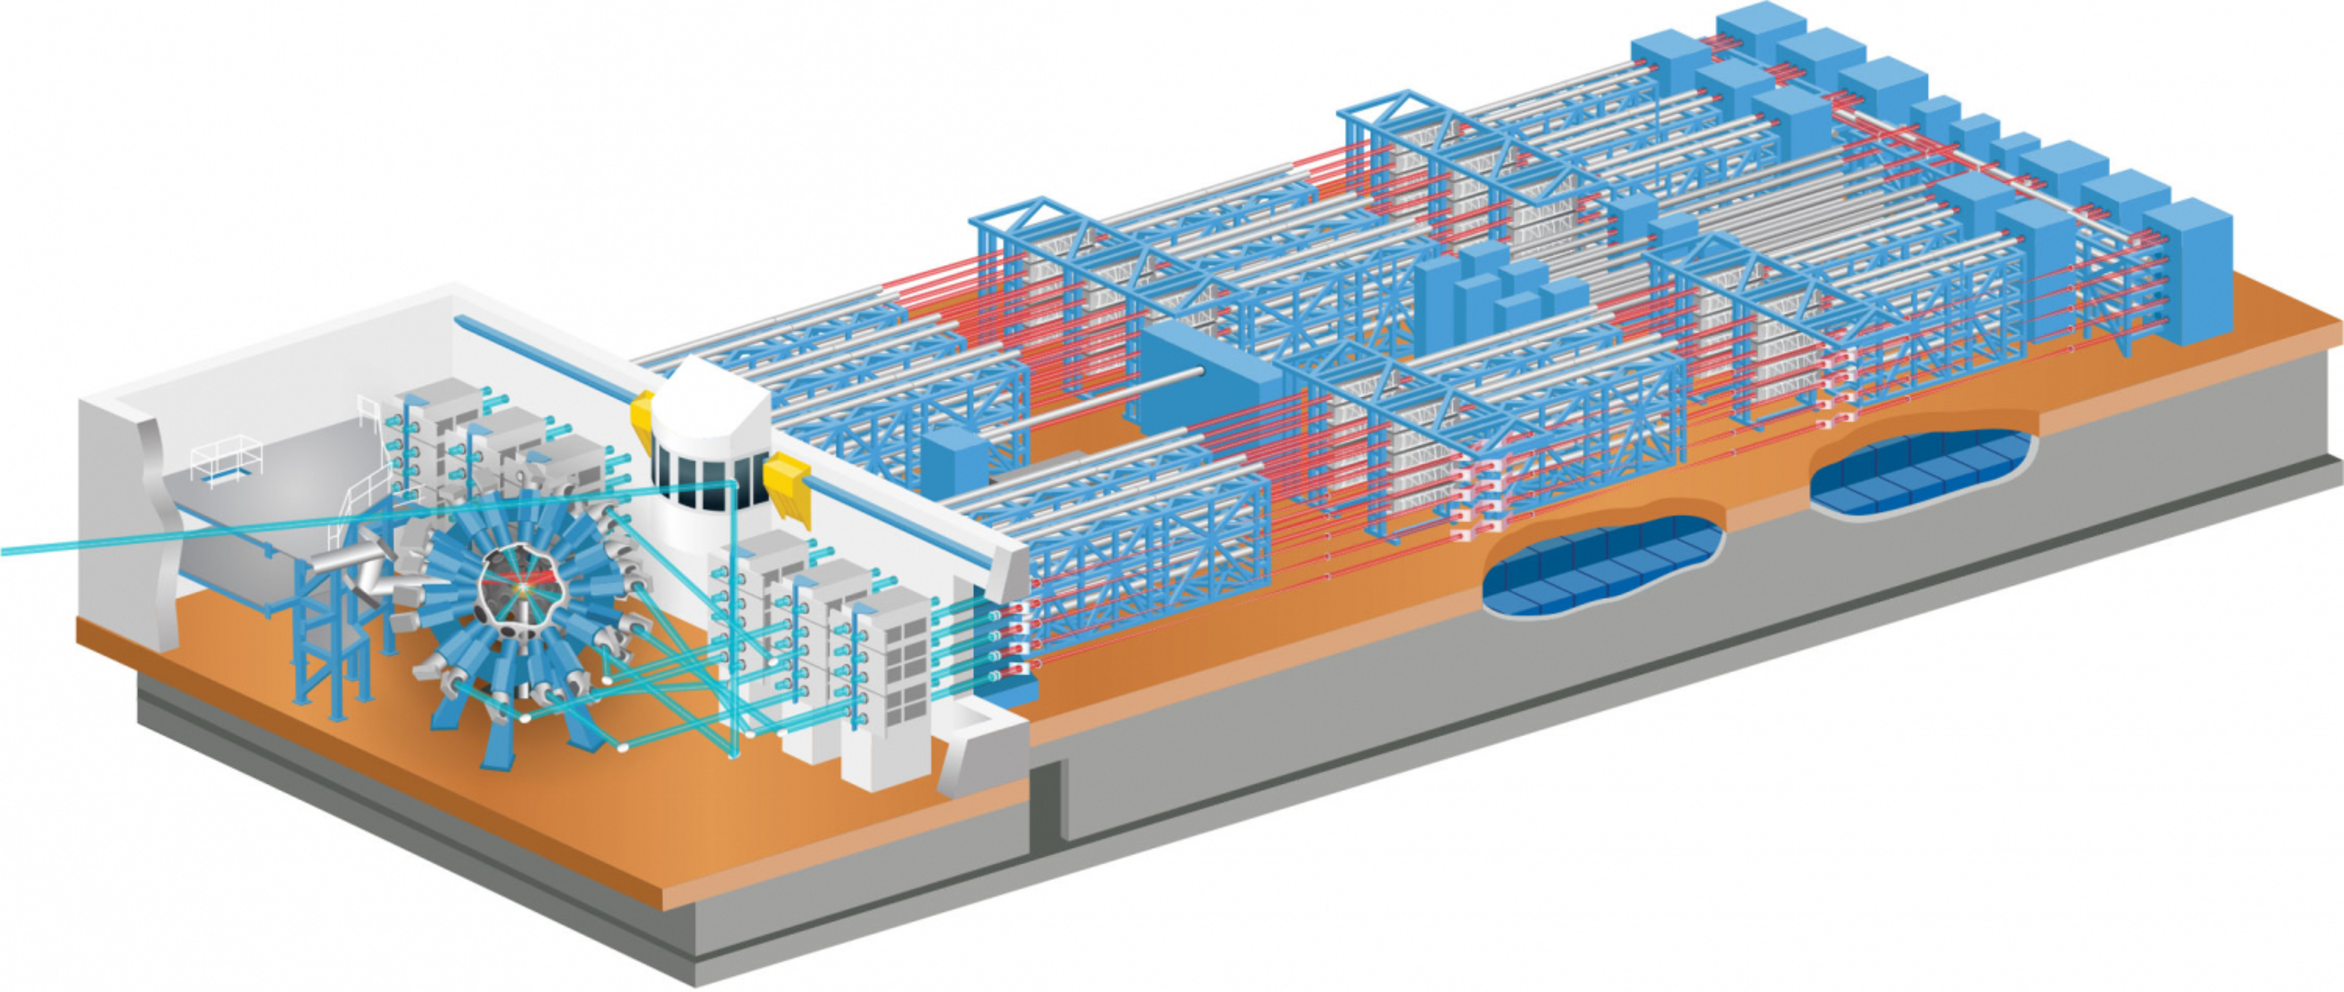
\includegraphics[scale=0.3]{Figures/omega60.pdf}
		\caption{\todo{OMEGA Laser} \cite{bibid}}
	\end{figure}

	The OMEGA laser was used for the Warm Dense Matter (WDM) stopping power experiments described in Chapter \ref{label}.
	
	
	
	
\subsection{The Z Pulsed Power Facility}
\label{sec:ZMachine}

The Z Pulsed Power Facility (informally known as the Z-machine or the Z) is the world's largest Z-pinch located in Albuquerque, NM operated by Sandia National Laboratories. It consists of 36 Marx Bank Generators that form a circle roughly 33 meters in diameter. Each have sixty 2.6 uF capacitors that are charged in parallel and discharged in series. Each generator can be discharged to generate a 150 kA current within 1.5 microseconds. The current travels through a series of intermediate capacitors that ultimately compress and combine the pulses to deliver currents between 10 to 26 MA with durations between 100 to 1000 ns. This facility is used for a vast variety of different experiments, but in our context, the current is delivered to a small cylindrical liner in the center of the machine. 

\begin{figure}[h!]
	\centering
	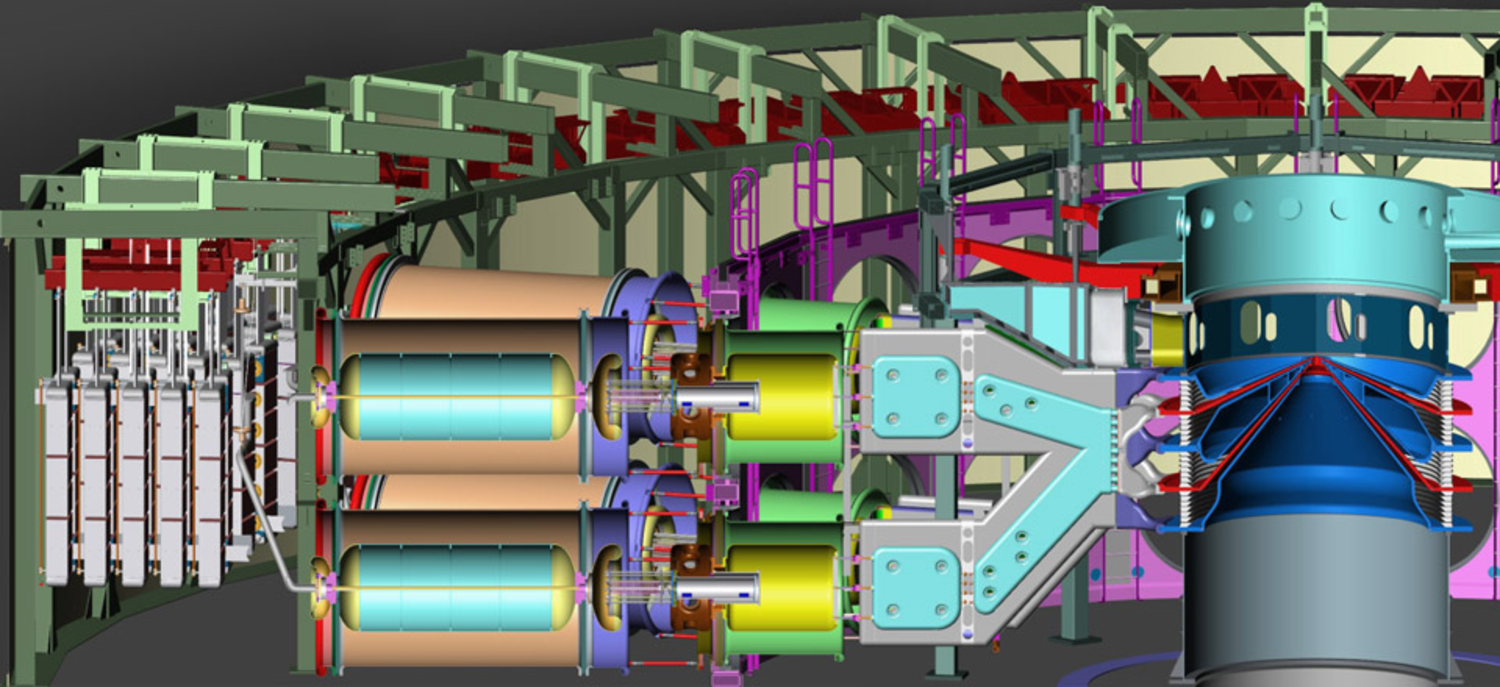
\includegraphics[scale=0.5]{Figures/zMachine.pdf}
	\caption{\todo{Z Machine} \cite{bibid}}
\end{figure}

The Z Pulsed Power facility was used for the experiments described in Chapter \ref{bibid}. The diagnostic discussed here was specifically made for the Z facility and will continue to see use beyond the work of this thesis. 





\subsection{The National Ignition Facility}
\label{sec:NIF}

The National Ignition Facility (NIF) is the world's most powerful laser located in Livermore, CA operated by Lawrence Livermore National Laboratory (LLNL). The NIF is an 192 beam laser capable of delivering 1.8 MJ at 500 TW. The beams are delivered through the top and bottom of a 10 meter diameter target chamber as opposed to the symmetric layout of the OMEGA laser. This is because the NIF is designed for the indirect drive approach to ICF discussed in Section \ref{sec:ICF}. Like the OMEGA facility, the NIF is equipped with a vast array of diagnostics that are either fixed to the target chamber or inserted prior to a shot.  

\begin{figure}[h!]
	\centering
	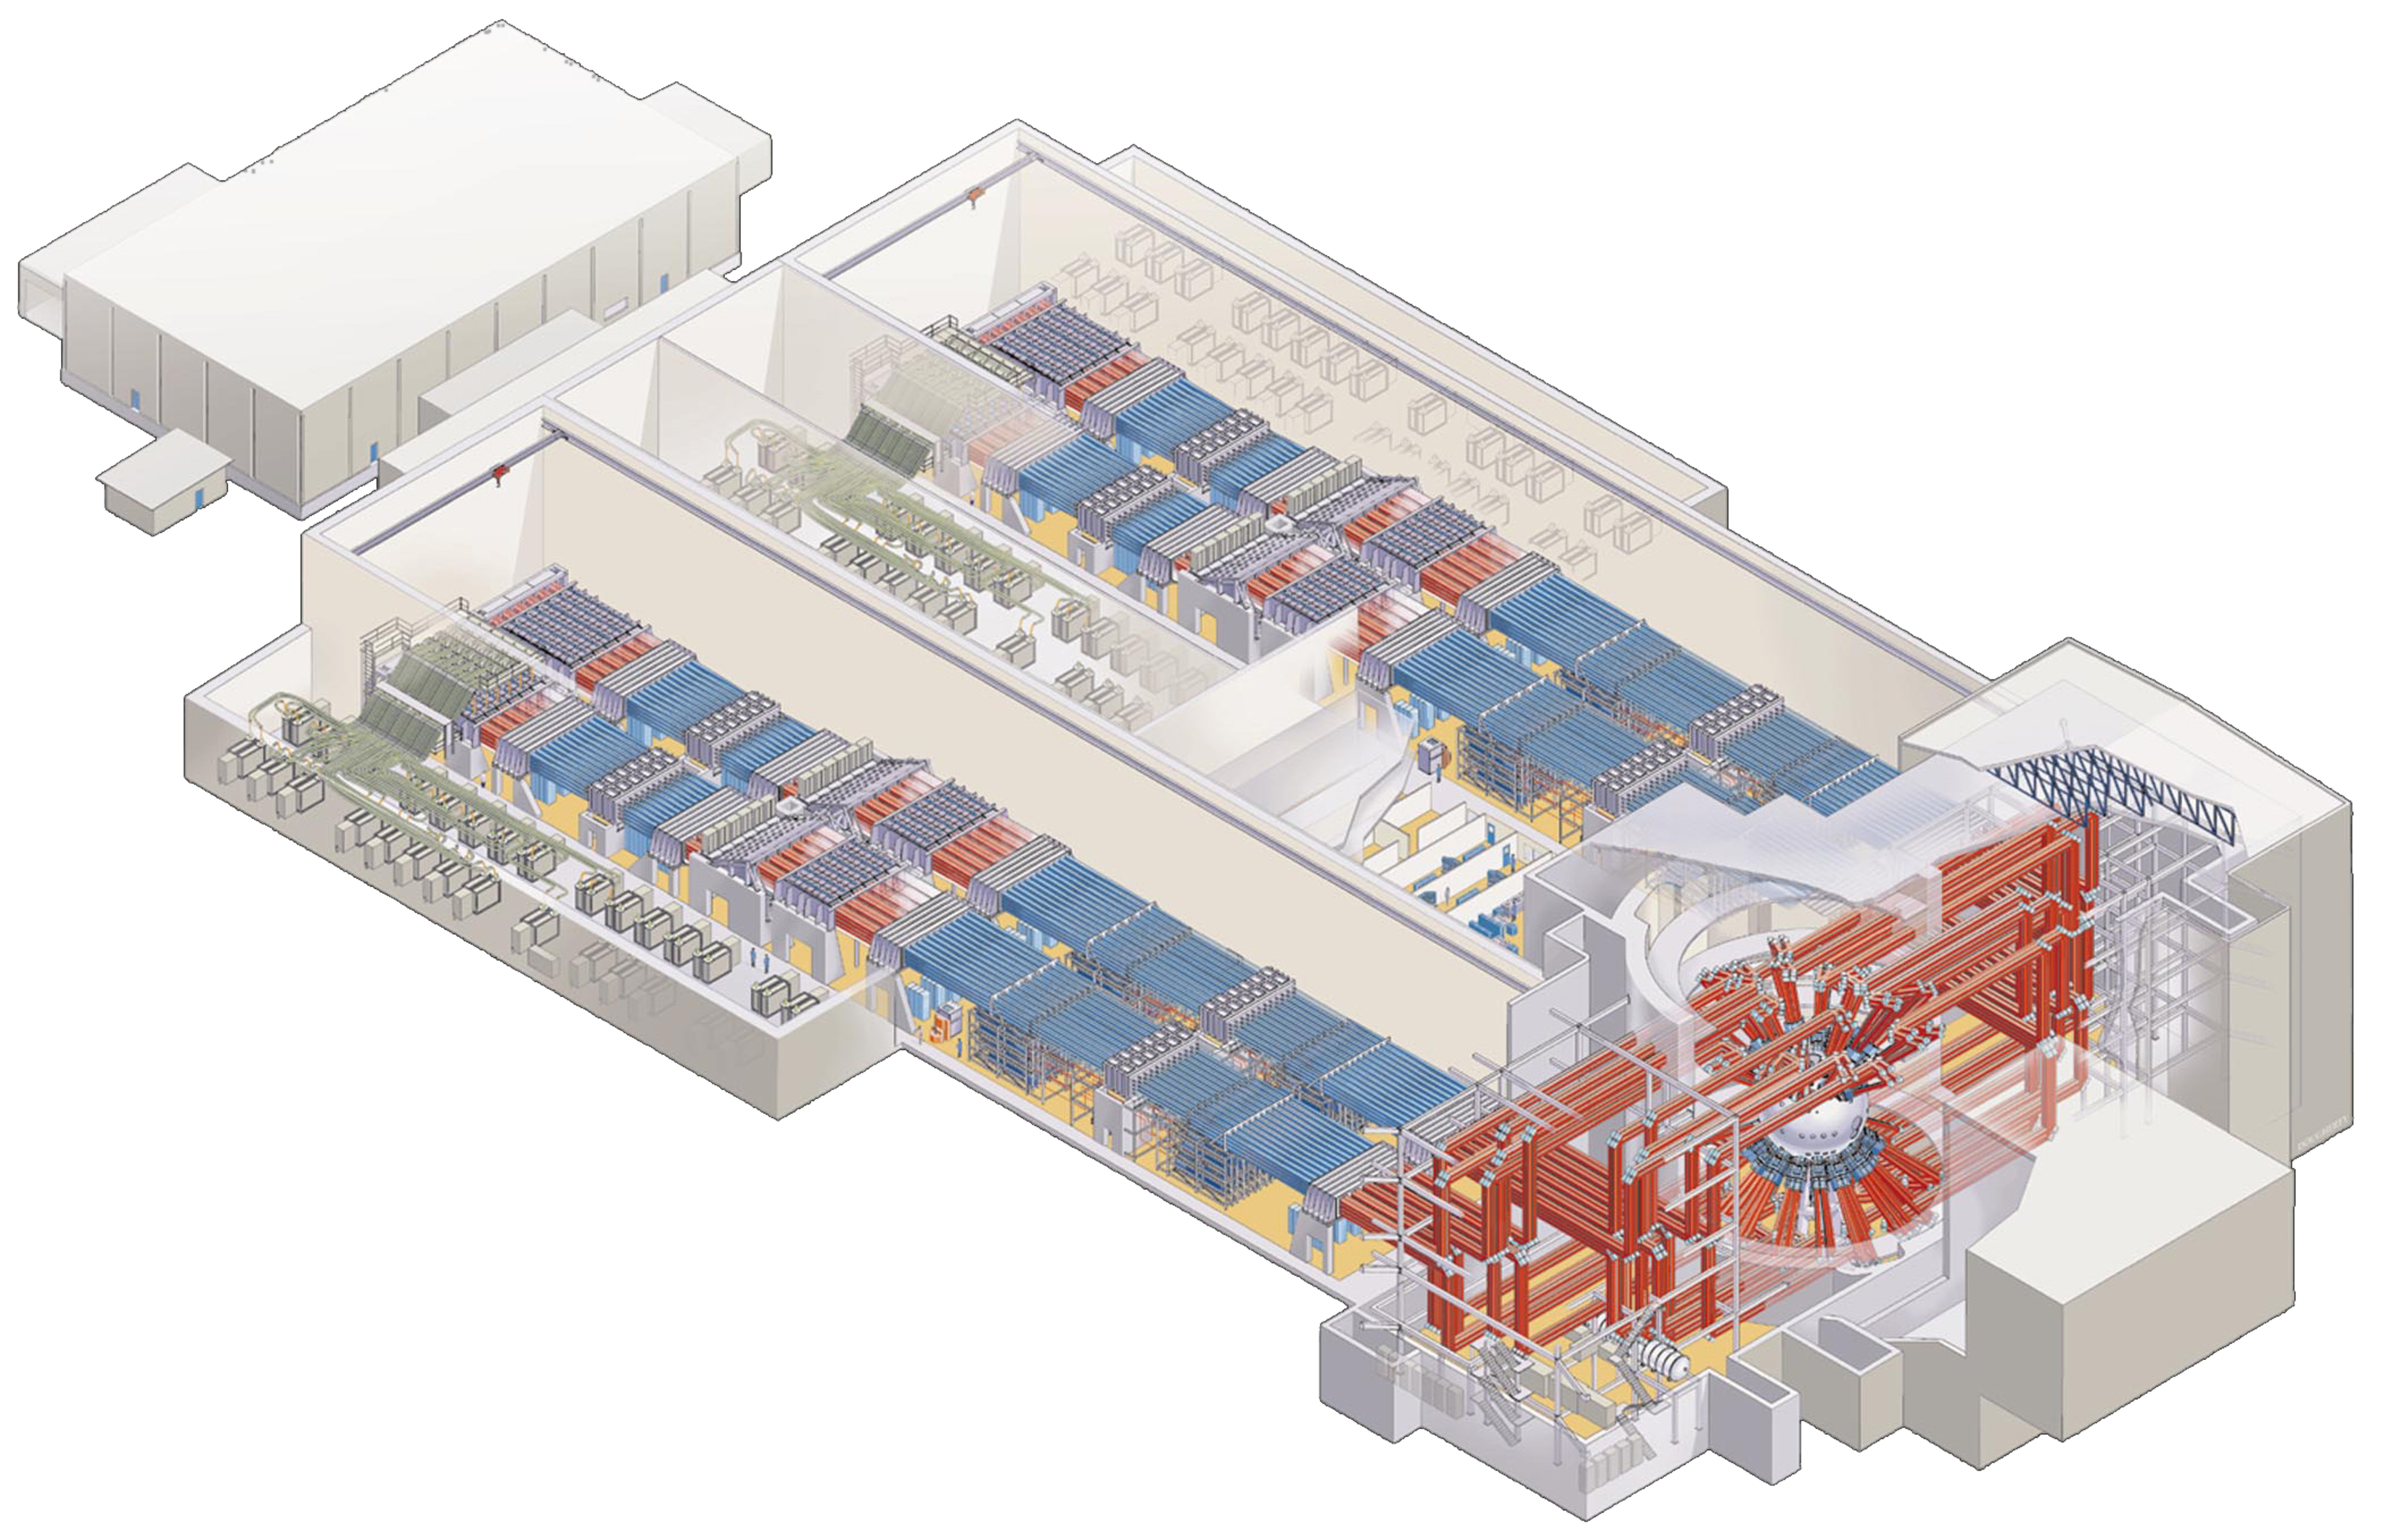
\includegraphics[scale=0.3]{Figures/theNIF.pdf}
	\caption{\todo{The NIF} \cite{bibid}}
\end{figure}

The work discussed in Chapter \ref{chap:secondaries} comes from a variety of experiments performed at the NIF. 



